\subsection{Differensforstærker}
\label{effekt_differensforstaerker}

\begin{figure}[h]
\centering
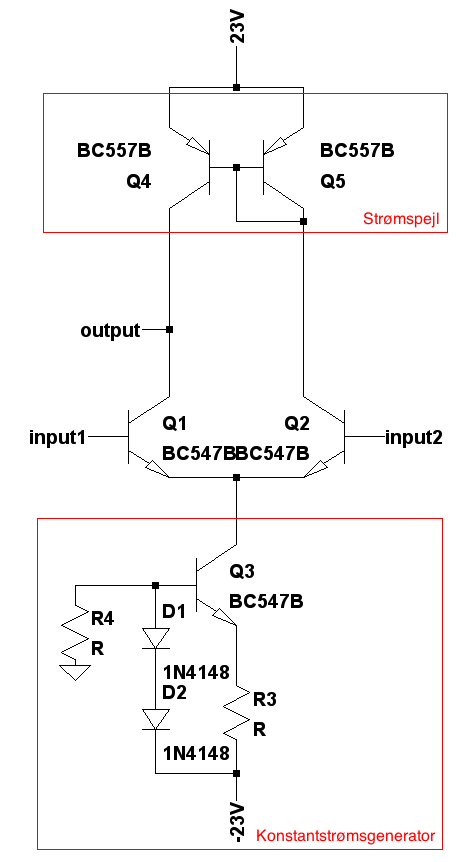
\includegraphics[scale=.4]{teknisk/effektforstaerker/differensforstaerker.png}
\caption{Diagram over differensforstærkeren hvor strømspejl og konstantstrømsgenerator er markeret}
\label{fig:differensforstaerker}
\end{figure}

Differensforstærkerens formål er at muliggøre tilbagekobling ved at forstærke forskellen mellem signalerne på input1 og input2, som vist på figur \ref{fig:differensforstaerker}, samt undertrykke common-mode signaler. Strømgeneratoren sørger for at der løber en konstant strøm, $\frac{1}{2}I_\mathrm{bias}$, i de to grene af differensforstærkeren når input1 = input2. For at disse strømme effektivt skal være ens er det nødvendigt at benytte matchede transistorer til både strømspejlet og Q1 og Q2. Stiger strømmen gennem Q2 med $\Delta I$, som følge af en øget spænding på input2 relativt til input1, vil strømspejlet øge strømmen i den modsatte gren så strømmene i de to grene er ens. Da der nu løber $\frac{1}{2}I_\mathrm{bias} + \Delta I$ i begge grene, men kun kan løbe $I_\mathrm{bias}$ gennem konstantstrømsgenerator vil der nødvendigvis løbe $I_\mathrm{bias} -\Delta I$ gennem Q1 og $2\Delta I$ ud i outputgrenen. Denne sammenhænge gælder både med en strømforøgelse og -formindskelse gennem Q2. På denne måde styres spændingsforstærkeren, som er dokumenteret i afsnit \ref{effekt_spaendingsforstaerker}. 

Biasstrømmen, $I_\mathrm{bias}$, som konstantstrømsgeneratoren skal generere vælges til 2 mA, da transistorparametrene for den anvendte transistor, BC547B (Q3), er veldefinerede ved denne collectorstrøm, hvilket letter beregningerne. Når der løber en strøm gennem generatoren på 2 mA vil der, hvis differensforstærkeren er i balance, løbe 1 mA i hver gren. Der antages at transistorparametrene angivet ved en collectorstrøm på 2 mA også er gældende for en strøm på 1 mA. 
Konstantstrømsgeneratoren designes ud fra samme procedure som benyttes i underafsnittet Konstantstrømsgenerator i afsnit \ref{effekt_stroemforstaerker}. $I_F$ aflæses i databladet for 1N4148 til 5 mA hvis en $V_F$ på 700 mV, hvilket er den nødvendige $V_\mathrm{BE}$ for Q3 for at opnå en collectorstrøm på 2 mA. Med denne procedure bliver strømgeneratorens komponentværdier som vist i ligning (\ref{eq:stroemdiff1}) og (\ref{eq:stroemdiff2}).

\begin{equation}
\label{eq:stroemdiff1}
R_4=\frac{23~\mathrm{V}-2 \cdot 0,7~V}{5~\mathrm{mA}}=4,32~\mathrm{k}\ohm
\end{equation}

\begin{equation}
\label{eq:stroemdiff2}
R_3=\frac{0,7~\mathrm{V}}{2~\mathrm{mA}}=350~\ohm
\end{equation}

For at kunne beregne CMRR, som er et udtryk for forholdet mellem differensforstærkningen og common-mode-forstærkningen, er der behov for netop at beregne disse forstærkninger. 
Differensforstærkningen, $A_d$, er et udtryk for hvor meget spændingsdifferensen mellem inputsignalet og det tilbagekoblede signal forstærkes. Ligning (\ref{eq:diffforstaerkning}) \cite{sedra-smith-2} %\fixme{kilde til sedra s. 618 eq 7.159}
er et udtryk for differensforstærkningen under antagelse af at hybrid-$\pi$~ parametrene for Q1, Q2, Q4 og Q5. Denne antagelse kan forekomme fordi strømmen i alle transistorerne er identisk når input1 = input2.

\begin{equation}
A_d=\frac{1}{2} \cdot g_m \cdot r_o
\label{eq:diffforstaerkning}
\end{equation}

Hybrid-$\pi$ parametren $g_m$ er givet ved $\frac{i_C}{V_T}$ og $r_o$ er givet ved $\frac{1}{h_\mathrm{oe} - g_m \cdot h_\mathrm{re}}$. H-parametrene $h_\mathrm{re}$ og $h_\mathrm{oe}$ er at aflæse i databladet, hvormed differensforstærkningen bliver som vist i ligning (\ref{eq:adberegning}).

\begin{equation}
A_d=\frac{1}{2} \cdot \frac{i_C}{V_T} \cdot \frac{1}{h_\mathrm{oe} - \frac{i_C}{V_T} \cdot h_\mathrm{re}}=367,6
\label{eq:adberegning}
\end{equation}

Differensforstærkningen ønskes høj så der er tilstrækkeligt at tilbagekoble. Givet at forstærkningen i spændingsforstærkeren er beregnet til 1964,44 gange anses $A_d$ for at være tilstrækkeligt. 

Common-mode-forstærkningen, $A_\mathrm{cm}$, er et udtryk for hvor meget et identisk signal på input1 og input2 vil bliver forstærket. $A_\mathrm{cm}$ ønskes så lav som muligt for f. eks. effektivt at kunne undertrykke indstrålet støj og DC. $A_\mathrm{cm}$ er givet ved ligning (\ref{eq:acmligning}) \cite{sedra-smith-3} %\fixme{kilde sedra s. 620 eq 7.165}
under antagelse af at transistorerne er perfekt matchede og  at $r_{o,Q4}>>r_{\pi,Q4},~r_{\pi,Q5}$. 

\begin{equation}
A_\mathrm{cm} = -\frac{r_o}{h_\mathrm{fe} \cdot R_E}
\label{eq:acmligning}
\end{equation}

Hvor $R_E$ er Q1 og Q2's emittermodstand som udgøres af konstantstrømsgeneratoren. Konstantstrømsgeneratorens impedans beregnes, som vist i (\ref{equ:spaendingsforstaerker3}) i afsnit \ref{effekt_spaendingsforstaerker}, hvormed den bliver $333~\mathrm{k}\ohm$. Dermed beregnes $A_\mathrm{cm}$ i ligning (\ref{eq:acmberegning}).

\begin{equation}
A_\mathrm{cm} = -\frac{\frac{1}{h_\mathrm{oe} - \frac{i_C}{V_T} \cdot h_\mathrm{re}}}{h_\mathrm{fe} \cdot R_E} = -0.17 \cdot 10^{-3}
\label{eq:acmberegning}
\end{equation}

I kravspecifikationen afsnit \ref{kravspecifikation} anses et signal dæmpet med 50 dB for slukket. Da forstærkningen beregnet i ligning (\ref{eq:acmberegning}) svarer til en dæmpningsfaktor på 75,2 dB, vurderes det at common-mode-forstærkningen er tilstrækkelig. 

Da $A_\mathrm{cm}$ og $A_d$ nu er beregnet, findes CMRR i ligning \ref{eq:cmrrberegning}.

\begin{equation}
\mathrm{CMRR}=20 \cdot \mathrm{log}_{10} \left( \frac{|A_d|}{|A_\mathrm{cm}|}\right)=126,5~\mathrm{dB}
\label{eq:cmrrberegning}
\end{equation}

For at have et grundlag for at vurdere den beregnede CMRR sammenlignes den med den for en operationsforstærker, LM324, da princippet i opbygningen er den samme. For operationsforstærkeren er CMRR opgivet til typisk at være 85 dB hvormed det vurderes at den beregnede er tilstrækkeligt. 

\subsubsection*{Analyse af ind- og udgangsimpedanser}
Til senere brug skal impedansen der kigges ind i på input2 samt impedansen der kigges ind i på output. 
Impedansen der kigges ind i på input2 er givet ved ligning (\ref{eq:input2impedans}) \cite{sedra-smith-4} %\kilde{sedra s. 734 figur 7.37b}
under antagelse af at hybrid-$\pi$~ paramtrene er ens for Q4, Q5, Q1 og Q2 samt at disse er perfekt matchede. 

\begin{equation}
R_{i, input2}= r_\pi = \frac{h_\mathrm{fe}}{\frac{i_C}{V_T}} = 8,58~\mathrm{k}\ohm
\label{eq:input2impedans}
\end{equation}

Impedansen der kigges ind i på output er givet ved ligning (\ref{eq:outputimpedansdiff}) \cite{sedra-smith-5} %\kilde{sedra s. 618  eq 7.157}
under samme antagelser som blev foretaget i ligning (\ref{eq:input2impedans}).

\begin{equation}
R_{o, output} = \frac{1}{2} \cdot r_o = \frac{1}{2} \cdot \frac{1}{h_\mathrm{oe} - \frac{i_C}{V_T} \cdot h_\mathrm{re}} = 9,56~\mathrm{k}\ohm
\label{eq:outputimpedansdiff}
\end{equation}
